%!TeX program = xelatex
\documentclass[12pt,a4paper,UTF8]{ctexart}
\usepackage{zjureport}
\usepackage{float}

\begin{document}

\cover
\clearpage

\pagenumbering{Roman}
\thispagestyle{empty}
\begin{abstract}
转座元件（transposable elements, TEs）是人类基因组的重要组成部分，能够通过插入突变、基因组重排、转录调控、表观遗传失衡和调控元件供给等方式影响基因组功能与疾病相关过程\cite{lander2001human,cordaux2009retrotransposons,chuong2017regulatory,bourque2018ten,burns2017cancer,payer2019genetic}。然而，TE 相关数据长期分散在重复序列注释、分类资源、表达矩阵、基因组位置、疾病文献和人工整理条目中。研究者若希望回答某一 TE 是否与疾病、功能或分子机制相关，往往需要在多个资源之间切换，并且难以追踪每一条关系背后的文献证据。本文构建 TE-KG，一个面向人类转座元件功能与疾病证据整合的知识图谱数据库。该数据库以医学文献数据库（PubMed）检索、TE 白名单、实体关系抽取、实体规范化、分类体系构建和图数据库整合为核心流程，并结合序列、基因组位置、表达数据、图谱浏览、路径探索和自然语言问答助手，为 TE 研究提供可浏览、可追踪和可复用的数据入口。当前数据构建流程从 34,788 篇人类 TE 相关候选文献出发，经白名单筛选和模型辅助抽取后保留 2,308 篇核心文献；运行图谱包含 11,415 个节点和 13,696 条有向关系，本地资源还包括 5,683,690 条重复序列注释记录、299 条 TE 分类记录、37,868 条表达浏览摘要、143 个表达上下文和 113,604 条表达数据集摘要。TE-KG 的定位不是自动给出未经审查的因果结论，而是以可追踪证据链支持 TE 疾病机制假设生成和数据库化复用。

\textbf{关键词：}转座元件；知识图谱；数据库；疾病证据；文献挖掘；智能问答
\end{abstract}

\clearpage
\tableofcontents

\clearpage
\pagenumbering{arabic}

\section{引言}

转座元件曾长期被视为重复序列或基因组噪声，但现代基因组学研究已经表明，它们是影响基因组结构、转录调控和疾病相关过程的重要组成部分。在人类基因组中，长散在核元件、短散在核元件、长末端重复序列来源元件和复合型逆转录转座元件等类别共同构成了大量重复序列。它们不仅记录了基因组演化历史，也可能通过提供启动子、增强子、剪接位点、转录因子结合位点和染色质调控信号参与宿主调控网络\cite{cordaux2009retrotransposons,chuong2017regulatory,bourque2018ten}。

TE 与疾病研究之间存在多种连接方式。部分 TE 插入事件可以直接破坏基因结构或改变转录产物，从而造成遗传病或增加疾病风险\cite{payer2019genetic}。在肿瘤中，某些逆转录转座元件会发生低甲基化和重新激活，可能促进插入突变、基因组不稳定和异常转录\cite{burns2017cancer}。内源性逆转录病毒来源序列和其他 TE 片段还可能参与免疫激活、病毒模拟反应和疾病状态下的调控重塑。由于这些过程横跨序列、位置、表达、功能、疾病和文献证据，TE 研究天然具有多层级和关系密集的特点。

现有资源为 TE 研究提供了重要基础，但通常服务于不同数据层。RepeatMasker、Repbase 和 Dfam 等资源支持重复序列注释、TE 家族模型和分类整理\cite{jurka2005repbase,smit2015repeatmasker,huber2016dfam,storer2021dfam}；PubMed 支持文献检索；表达数据资源支持转录活跃性观察；疾病或基因数据库支持特定实体查询。对于单点查询而言，这种分工是有效的；但对于机制性问题而言，研究者常常需要把多个层面的证据重新拼接。例如，若用户希望理解 L1HS 与癌症之间的关系，仅知道其分类或序列并不足够；用户还需要知道相关关系来自哪些文献、是否涉及插入突变或低甲基化、相关基因或功能是什么、表达证据是否支持该背景，以及这些证据能否导出并复查。

知识图谱适合表达这种多源异构证据。生物医学知识图谱已经被用于连接疾病、基因、药物、表型和文献，从而支持关系浏览、证据整合和假设优先级排序\cite{himmelstein2017hetionet,chandak2023building,huber2023kghub,morris2023spoke,sumer2021crossbar}。对于 TE 研究而言，知识图谱的价值不在于替代生物学实验，也不在于自动判定因果强度，而在于把 TE、疾病、功能、基因、蛋白、RNA、表达上下文和文献证据放入同一可追踪网络。用户可以沿图谱边检查证据来源，而不是在孤立表格和文献摘要之间反复切换。

本文介绍 TE-KG，一个面向人类 TE 功能与疾病证据整合的知识图谱数据库。该数据库整合三类能力：第一，围绕 TE 实体组织分类、序列、位置和表达上下文；第二，从文献和结构化数据中整理 TE 与疾病、功能、基因和分子实体之间的关系；第三，通过网页界面和自然语言问答助手支持用户进行证据查询、图谱探索和结果导出。

\section{材料与方法}

\subsection{文献检索与候选文章收集}

TE-KG 的文献数据构建以 PubMed 为主要入口。检索式结合医学主题词和自由词，覆盖 ``DNA Transposable Elements''、``retrotransposon''、``transposon''、``retrotransposons''、``transposons''、``Retrotransposition'' 和 ``transposition'' 等术语，并限定在人类或智人相关语境中。根据数据构建记录，检索覆盖截至 2026 年 4 月 13 日的文献，共获得 34,788 篇候选文章。该检索策略的目的不是在第一步获得完全精确的 TE 文章集合，而是先形成较高召回率的候选文献池，再通过 TE 名称白名单、模型辅助抽取和人工验证逐步提高特异性。

每条文献记录至少保留 PMID、标题、摘要、发表年份和期刊信息。由于 PubMed 主要提供文献元数据和摘要入口，而不提供期刊影响因子等评价指标\cite{pubmed_ncbi}，TE-KG 在数据设计中将文献证据与期刊元数据分开处理。关系是否有文献支持，取决于是否存在可追踪的 PMID 和对应文本证据；期刊层面的附加信息只能作为辅助元数据，不能替代关系本身的证据判断。

\subsection{人类 TE 白名单构建}

候选文献检索之后，TE-KG 构建了用于筛选和实体触发的人类 TE 白名单。该白名单主要来自两类资源：一类是 RepeatMasker 注释中的人类 TE 名称，另一类是 Repbase 中的人类 TE 标识符及关键词行文本\cite{jurka2005repbase,smit2015repeatmasker}。白名单的功能是为标题、摘要和模型输出提供候选 TE 名称约束，从而降低普通词汇、非人类物种 TE 和宽泛机制词造成的误匹配。

白名单本身并不被视为最终事实来源。不同资源中的 TE 命名粒度不同，同一元件可能同时以家族、亚家族、共识序列或注释名称出现；部分名称还可能与普通英文词或其他生物学术语重合。因此，白名单被用于候选识别和筛选，而最终进入图谱的实体仍需要经过规范化和人工校正。

\subsection{文献筛选与实体关系抽取}

TE-KG 采用两阶段筛选流程。第一阶段使用白名单在候选文章标题和摘要中进行匹配，从初始候选集中保留 5,362 篇可能讨论人类 TE 的文章。随后，系统调用大语言模型对这些文章进行结构化信息抽取，要求模型识别与人类 TE 相关的实体和实体关系，并按照固定结构输出结果。第二阶段再次基于白名单检查模型输出，排除没有识别到人类 TE 实体的文章，最终保留 2,308 篇核心文章。同时，1,803 篇文章被标记为可能存在 TE 遗漏，用于后续人工检查和误差分析。

抽取对象包括 TE、疾病、功能、突变、基因、RNA、蛋白、糖类、脂类、肽类、药物和毒素等实体类型。关系被组织为因果关系、调控关系、相互作用、关联关系和遗传信息流关系五类语义框架。为降低自由生成带来的不可控性，抽取提示词约束模型输出为固定结构，并要求每篇文章中的同一实体只出现一次。模型输出不是直接等同于最终事实，而是作为候选结构化记录，后续仍需接受白名单检查、实体规范化和人工质量评估。

\subsection{实体规范化与分类体系构建}

实体规范化是 TE-KG 构建中的关键步骤。TE 名称可能存在大小写差异、标点差异、资源命名差异和分类粒度差异；疾病、功能、基因和分子实体也可能存在同义词或缩写。为减少重复节点和关系碎片化，TE-KG 对同类型实体采用 Ratcliff/Obershelp 字符串相似度方法进行聚类，相似度阈值设为 80\%\cite{ratcliff1988pattern}。聚类结果随后经过人工校正，用于建立同义词到规范名称的映射。

TE 分类体系主要基于 Repbase 注释；对于 Repbase 中未记录或分类不完整的 TE，使用 RepeatMasker 分类作为补充。为兼顾分类严谨性和图谱覆盖度，TE-KG 构建两套层级树：第一套仅包含在 Repbase 或 RepeatMasker 中有明确注释的 TE；第二套以第一套为基础，纳入知识图谱中出现的全部 TE 实体。疾病分类体系以国际疾病分类第十一次修订版为主要参考\cite{icd11_who}，并对难以归入单一主类的疾病或表型设置辅助分支，以服务检索和浏览。

\subsection{知识图谱构建}

TE-KG 采用图数据库组织实体与关系。图数据库适合表达多类型节点和多跳关系，并支持从某个 TE 出发追踪疾病、功能、基因、文献和表达上下文之间的连接\cite{neo4j_graph}。图谱节点包括 TE、疾病、功能、突变、基因、RNA、蛋白、药物、毒素和文献等类型。关系记录保留来源实体、目标实体、关系语义、描述、证据来源和 PMID 追踪字段。

图谱构建遵循证据优先原则。TE-KG 不把文献数量、期刊元数据或模型判断直接等同于因果强度，而是把它们拆分为可检查字段。用户在浏览某条关系时，应能够看到该关系对应的来源文献、抽取描述和相关实体，而不是只看到一个不可解释的分数。这样的设计有利于后续人工审查、导出复用和版本更新。

\subsection{序列、基因组位置和表达数据整合}

除了文献关系，TE-KG 还整合了 TE 研究所需的基础上下文。序列层面用于提供共识序列、长度和来源说明；基因组位置层面用于提供代表性位点或注释记录；表达层面用于描述 TE 在不同组织、细胞系或疾病相关样本中的表达分布。当前本地数据中，RepeatMasker 注释文件包含 5,683,690 条记录；TE 分类表包含 299 条记录；表达模块包含 37,868 条浏览摘要、143 个表达上下文和 113,604 条数据集摘要。

这些数据层在图谱中承担不同角色。序列和位置帮助用户确认 TE 实体的基础属性；表达数据帮助用户判断某个 TE 是否在特定组织或细胞背景下具有活跃性；文献关系帮助用户追踪 TE 与疾病、功能和分子实体之间的证据。TE-KG 的核心价值正在于把这些层次连接起来，使用户能够从一个 TE 条目进入多维证据空间。

\subsection{网页平台和智能问答助手实现}

TE-KG 提供面向研究者的网页入口。实体浏览页面支持用户按名称、分类和关键词查找 TE；图谱页面支持用户查看局部关系网络、展开节点和检查边信息；路径探索页面支持用户查询 TE、疾病、基因或功能之间的连接路径；表达页面支持用户查看不同数据集和上下文中的 TE 表达模式；下载页面支持用户获取可复用数据表。

TE-KG 还提供自然语言问答助手，用于帮助用户以普通问题访问数据库证据。问答助手将用户问题解析为实体、意图和所需证据层，再调用分类、序列、基因组位置、表达、图谱关系、文献和引用等数据模块，最后由模型整合为自然语言答案。它不是原始科学证据来源，也不替代人工判断；它是数据库证据的检索、整合和解释入口。

\subsection{质量控制与人工验证}

文献筛选质量通过人工抽样进行评估。人工复核覆盖三组文章：第一组为初筛阶段移除的 27,108 篇文章，第二组为二次筛选阶段移除的 5,362 篇文章，第三组为图谱整合阶段标记的 1,803 篇疑似遗漏文章。每组随机抽取 50 篇文章进行人工检查。初筛移除文章的正确过滤率为 100\%，二次筛选移除文章的正确过滤率为 94\%，整合阶段标记文章的判断正确率为 96\%。

置信区间估计进一步说明了筛选流程的可靠性。初筛移除组使用 Clopper--Pearson 精确方法估计 95\% 置信区间，为 92.9\% 至 100\%；二次筛选组和整合标记组使用 Wilson 区间，分别为 83.78\% 至 97.94\% 和 93.19\% 至 97.9\%。错误来源主要包括部分人类 TE 未出现在 Repbase 或 RepeatMasker 白名单中，以及模型在抽取阶段遗漏了真实 TE 实体。

\section{结果}

\subsection{TE-KG 的总体描述}

TE-KG 是一个面向人类 TE 的知识图谱数据库，整合文献证据、图谱关系、TE 分类、序列、基因组位置、表达数据和网页交互功能。数据库提供 Home、Browse、TE-KG、Path Finder、Expression、Agent 和 Download 等入口，使用户可以从 TE 名称、疾病实体、表达上下文或自然语言问题进入同一套证据体系。

TE-KG 的设计目标是把研究者常见的 TE 问题组织为可追踪数据查询。例如，用户可以先从 Browse 页面进入某个 TE 条目，再跳转到图谱页面查看疾病或功能关系，也可以在表达页面检查不同组织或细胞系背景下的表达模式。对于综合性问题，用户还可以使用问答助手汇总分类、序列、位置、表达和文献证据。

\subsection{数据组成与图谱规模}

当前运行图谱包含 11,415 个节点和 13,696 条有向关系，其中 2,308 个文献节点用于记录 PMID 级证据。由于文献节点承担证据索引功能，而不是普通生物实体，本文在实体组成图中排除了文献节点。剔除文献节点后，图谱中的主要实体类型包括功能、基因、蛋白、疾病分类、疾病、RNA、突变、药物和 TE 等。关系组成显示，调控、导致、表达、抑制、影响、介导、编码、相互作用、促进、插入和激活等具体谓词是当前较常见的关系表达方式。

\begin{figure}[htbp]
\centering
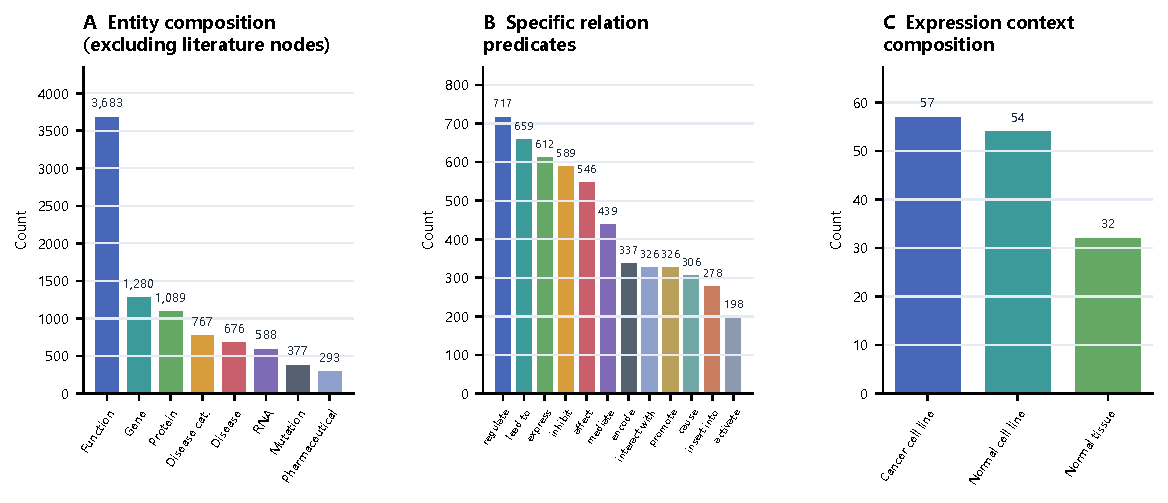
\includegraphics[width=0.98\textwidth]{figures/generated/figure2_data_composition.pdf}
\caption{TE-KG 数据组成。A，实体组成，文献节点未纳入统计，仅展示频数较高的真实实体类型。B，具体关系谓词组成，仅展示选定的高频或生物学语义明确的真实关系谓词，未展示低频或过泛谓词。C，表达数据上下文组成，统计单位为表达上下文而非表达记录数。}
\label{fig:data-composition}
\end{figure}

除图数据库外，TE-KG 还组织了多个辅助数据层。文献构建流程从 34,788 篇候选文章出发，经白名单筛选保留 5,362 篇候选文章，并在模型辅助抽取和二次筛选后保留 2,308 篇核心文章。本地数据还包括 5,683,690 条重复序列注释记录、299 条 TE 分类记录、37,868 条表达浏览摘要、143 个表达上下文和 113,604 条表达数据集摘要。这些数据共同构成 TE-KG 的可查询基础。

\subsection{实体浏览与 TE 分类探索}

Browse 页面为用户提供实体级访问入口。用户可以通过搜索框、分类筛选和条目列表定位目标 TE，并查看其分类、别名、描述和相关上下文。TE 分类树主要用于帮助用户从大类、家族或亚家族层面理解目标 TE 的位置。与只给出表格结果的数据库不同，TE-KG 的浏览入口还连接到图谱、表达和问答模块，使用户能够从一个条目继续进入关系网络。

分类浏览的价值在于降低 TE 命名复杂性带来的检索门槛。不同资源中，同一 TE 可能以不同粒度或别名出现。TE-KG 在浏览层保留规范名称和别名映射，使用户能够在不熟悉完整命名体系的情况下找到目标条目。对于分类不完整或需要进一步审查的 TE，系统应保留来源和状态信息，避免把候选分类误写成稳定结论。

\begin{figure}[htbp]
\centering
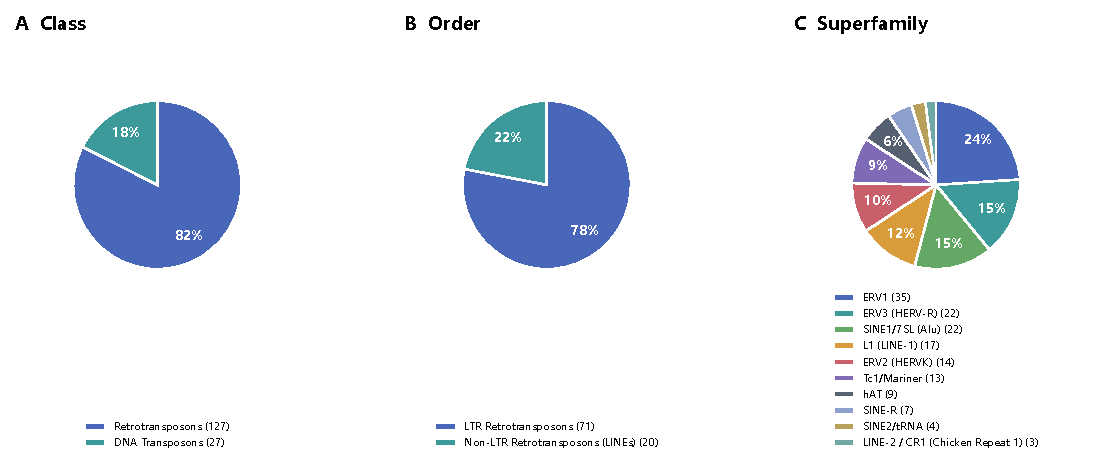
\includegraphics[width=0.98\textwidth]{figures/generated/figure3_te_classification_pies.pdf}
\caption{TE 分类层级组成。A，Class 层级。B，Order 层级。C，Superfamily 层级。Superfamily 面板仅展示频数较高的真实类别，低频类别未在图中展示。}
\label{fig:te-classification}
\end{figure}

\subsection{知识图谱可视化与关系探索}

TE-KG 图谱页面用于展示 TE 与疾病、功能、基因、RNA、蛋白和文献证据之间的关系。用户可以加载局部网络、展开节点、检查边信息，并在证据表中查看关系描述和文献来源。

图谱可视化的重点不是给出自动化因果判断，而是把关系和证据同时暴露给用户。若某个 TE 与疾病存在关系，用户需要知道该关系是插入事件、表达异常、低甲基化、一般关联还是其他机制线索，并进一步检查 PMID 记录。这样的设计可以减少将“有文献记录”误读为“机制已被证明”的风险。

\subsection{路径探索与疾病证据链追踪}

Path Finder 页面用于查询两个实体之间的连接路径。对于 TE 疾病机制研究，路径探索可以帮助用户回答“某个 TE 如何通过功能或基因连接到疾病”这类问题。路径结果本身并不等同于生物学因果链，但可以作为假设生成和证据审查的入口。用户应逐条检查路径中的关系和文献来源，而不是把整条路径视为同等强度的证据。

路径探索尤其适合多跳问题。例如，用户可以从 TE 出发，经过功能或基因节点追踪到疾病实体；也可以从疾病出发，回溯到相关 TE 和分子事件。与单表检索相比，路径视图更适合呈现间接连接，但也更需要明确证据边界。因此 TE-KG 在设计中强调路径可视化与证据表并行展示。

\subsection{表达模块与多层证据整合}

Expression 页面提供 TE 表达层面的上下文。当前表达数据覆盖正常组织、正常细胞系和癌症细胞系三类上下文，共 143 个表达上下文。表达模块不直接证明 TE 与疾病之间存在因果关系，但可以帮助用户判断某个 TE 是否在特定组织、细胞系或疾病相关背景下具有表达活跃性。

表达数据与图谱关系结合后，可以支持更具体的数据库查询。例如，若某个 TE 在癌症细胞系中具有较高表达，同时图谱中存在与癌症相关的文献关系，用户可以进一步检查该关系的 PMID 支持、关系类型和涉及的基因或功能节点。这样的多层证据整合比单独查看表达矩阵或文献列表更适合数据库化探索。

\subsection{面向证据检索的自然语言问答助手}

TE-KG 的自然语言问答助手用于把普通语言问题转化为数据库证据检索。用户可以询问某个 TE 的序列长度、代表性位置、表达组织、疾病关系或综合信息。系统先解析问题中的实体和意图，再调用相应数据模块，最后生成带证据边界的回答。问答助手降低了数据库使用门槛，但其回答仍应回到数据库记录和 PMID 证据进行核验。

问答助手的一个重要设计原则是区分证据和解释。图谱关系、文献记录和表达摘要属于数据库证据；模型生成的自然语言回答属于证据整理。对于证据不足的问题，系统应明确指出缺口，而不是用模板化语言补齐缺失结论。对于中文问题，问答过程和最终回答也应保持中文，以减少中英文夹杂造成的理解障碍。

\subsection{生物学应用案例}

L1HS 是 TE-KG 中适合作为示例的代表性 TE。围绕 L1HS，用户可以同时查看序列、代表性基因组位置、疾病关系、文献证据、表达上下文和问答助手整合结果。当前数据库中，L1HS 的共识序列长度为 6,064 bp，并有代表性位置记录 chr1:231646101--231652225。图谱关系将 L1HS 与癌症、癌、结直肠癌、肺癌、精子发生异常和其他疾病实体连接起来；相关证据需要通过边记录和 PMID 进一步核验。

\begin{figure}[H]
\centering
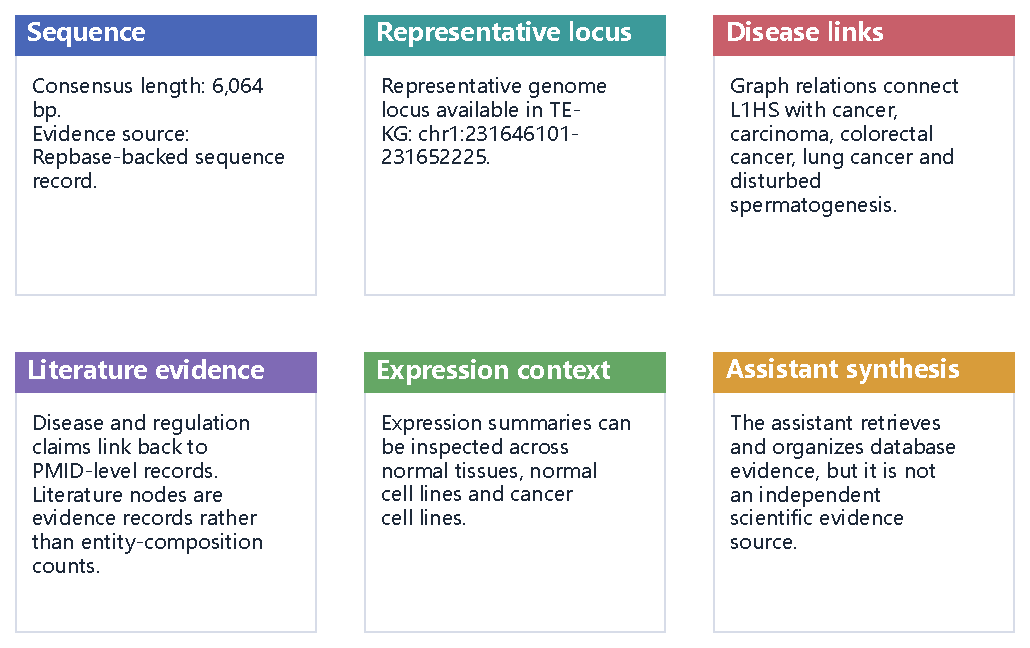
\includegraphics[width=0.98\textwidth]{figures/generated/figure4_l1hs_case.pdf}
\caption{L1HS 应用案例。该图以证据卡片方式展示 L1HS 的序列、代表性位置、疾病关系、文献证据、表达上下文和问答助手整合结果。该图不表示因果流程，所有疾病关系仍需回到数据库边和 PMID 记录核验。}
\label{fig:l1hs-case}
\end{figure}

该案例说明 TE-KG 的核心使用方式：用户不必把序列库、文献检索、表达矩阵和图谱工具分开使用，而可以从一个 TE 实体进入多层证据空间。对于 L1HS 这样的活跃人类特异性 LINE-1 亚家族，数据库化整合有助于快速整理候选机制，但最终解释仍需要结合原始文献和实验背景。

\section{讨论}

TE-KG 的主要价值在于把人类 TE 相关证据组织为可浏览、可追踪和可导出的知识图谱数据库。与只提供序列、注释或文献列表的资源相比，TE-KG 更强调关系层面的证据组织：用户不仅能看到某个 TE 的基础属性，也能看到它与疾病、功能、基因、表达和文献之间的连接。这种设计适合支持 TE 疾病机制研究中的假设生成和证据审查。

TE-KG 也与通用生物医学知识图谱形成互补。通用知识图谱通常覆盖大量疾病、药物、基因和表型实体\cite{himmelstein2017hetionet,chandak2023building,huber2023kghub,morris2023spoke}，但未必围绕 TE 命名、TE 分类、重复序列注释和 TE 表达上下文进行专门组织。TE-KG 将 TE 作为中心实体，能更细致地处理 TE 命名、分类和文献关系中的特殊问题。

自然语言问答助手是 TE-KG 的重要使用入口，但它必须受到证据边界约束。模型可以帮助用户整理数据库证据、合并多层信息和生成可读摘要，却不能替代原始文献或实验验证。本文将问答助手定位为数据库接口，而不是独立证据来源。这个定位对于避免过度解释尤其重要。

TE-KG 仍存在局限。首先，文献抽取主要依赖标题和摘要，可能遗漏全文中才出现的细节关系。其次，白名单策略可能漏掉资源中未收录或命名不一致的人类 TE。第三，大语言模型抽取存在方向错误、实体边界错误和共现误判为关系的风险。第四，图谱关系表示“存在可追踪记录”，并不自动表示因果机制已经被证明。后续版本需要补充更多人工复核、全文证据、版本化发布和可复现统计。

\section{结论}

本文构建了 TE-KG，一个面向人类 TE 功能与疾病证据整合的知识图谱数据库。该数据库从 34,788 篇候选文献出发，结合 TE 白名单、模型辅助抽取、实体规范化、分类体系和图数据库构建，将 TE 基础属性、疾病关系、功能关系、表达上下文和文献证据组织到同一可追踪框架中。TE-KG 通过图谱浏览、路径探索、表达查询、数据下载和自然语言问答助手，为研究者提供了从 TE 实体出发审查多层证据的入口。后续工作将继续完善公开数据版本、关系抽取质量评估、更多案例分析和长期更新机制。

\reference

\end{document}
